\documentclass[10pt]{article}
\usepackage[margin = 0.75in]{geometry}
\usepackage[onehalfspacing]{setspace}
\usepackage[hidelinks]{hyperref}
\usepackage[sfdefault]{noto}
\usepackage[T1]{fontenc}
% \usepackage[hangul]{kotex} % Korean Version
\usepackage{graphicx, fontawesome, calc, enumitem}
\setlength{\parindent}{0pt}
\setlength{\tabcolsep}{0pt}
\setlist[itemize, 1]{leftmargin = 0.1in}
\setlist[itemize, 2]{leftmargin = 0.3in}
\NewDocumentCommand \TIME { m o } {#1\IfValueTF{#2}{\newline \enspace to #2}{}}
\NewDocumentCommand \HEAD { m } {\raggedleft \textbf{#1} \qquad}

\begin{document}
  \pagestyle{empty}

  \begin{tabular}{ p{.75\linewidth} p{.25\linewidth} }
    % Name
    {\Large Paul Kim} \newline
    % One-Liner Description
    % Computer Engineer and Software Developer
    Undergraduate at Electrical \& Computer Engineering,
    Seoul National University \newline
    % Social and Background
    \faLinkedin{} \href{https://www.linkedin.com/in/thekpaul}{@thekpaul} \quad
    \faHome{} \url{https://thekpaul.dev} \quad
    \faFlag{} Republic of Korea \newline
    \faGithub{} \href{https://www.github.com/thekpaul}{thekpaul} \quad
    \faInstitution{} \href{mailto:jsvn7777@snu.ac.kr}{jsvn7777@snu.ac.kr} \quad
    \faEnvelopeO{} \href{mailto:thekpaul000@gmail.com}{thekpaul000@gmail.com}
    &
    % Profile Picture
    \multicolumn{1}{r}{\raisebox{-\height+11pt}{%
      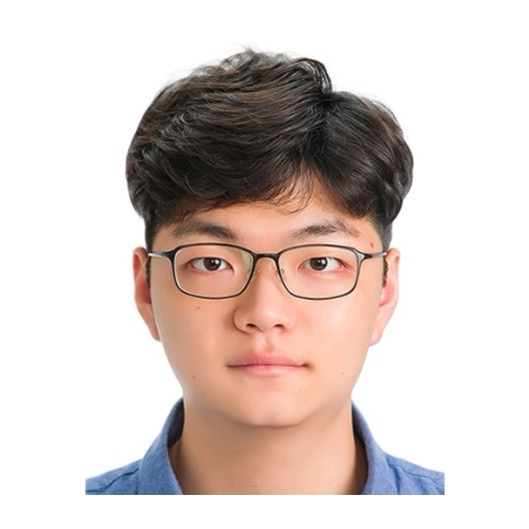
\includegraphics[width = .25\linewidth]{../refs/mugshot.png}}}
  % \vspace{10pt}
    \\ \hline
  \end{tabular}

  \begin{center}
    \begin{tabular}{ p{.2\linewidth}  p{.8\linewidth}}
      {\Large Education} & \\[10pt]
      \TIME{Mar. 2018} &
        {\large BA in Electrical \& Computer Engineering,
        Seoul National University} \newline
        Expected to graduate in Summer 2024 \newline
        \textbf{Areas of Interest}: System Programming, Digital Systems Design,
          Deep Learning \newline
        \textbf{Graduation Project}: Optimising the CNN Architecture with
          Hardware Design
      % \\[5pt]
    % \TIME{Mar. 2015}[Feb. 2018] &
    %   {\large Sangmoon High School}
      \\[10pt]
      {\Large Experience} & \\[10pt]
      \TIME{Mar. 2023} &
        {\large FPGA Engineer Intern for \textbf{NeuroRealityVision}} \newline
        Dongtan, Republic of Korea
        \begin{itemize}
          \item Firmware-based development for MIPI and Ethernet Integration
          \item Bare-metal, standalone FPGA application with interrupt-based
            workflow
        \end{itemize}
      \\[-5pt]
      \TIME{Jan. 2023}[Jun. 2023] &
        {\large Student Intern for Dept. of System Semiconductor Engineering}
        \newline
        \textbf{Seoul National University}, Seoul, Republic of Korea
        \begin{itemize}
          \item Worked on CNN Architecture and Hardware Design Optimisation
        \end{itemize}
      \\[-5pt]
      \TIME{Dec. 2019}[Jul. 2021] &
        {\large KATUSA, Human Resources Specialist (42A)} \newline
        \textbf{94\textsuperscript{th} Military Police Battalion},
        Pyeongtaek, Republic of Korea
        \begin{itemize}
          \item Mandatory military service as a KATUSA Agent \newline
            (Korean Augmentation To the United States Army)
        \end{itemize}
      \\[5pt]
    % {\Large Publications} & \\[10pt]
    % \TIME{<++>} &
    %   <++>
    % \\[20pt]
      {\Large Skills} & \\[10pt]
      \HEAD{Engineering} & \vspace{-\baselineskip}
        \begin{itemize}
          \item Experienced in embedded systems design on multi-purpose
            SoC FPGAs
          \item Capable of versatile development with C, C++ and Python
          \item Capable of basic RTL hardware design using Verilog
          \item Capable of maintaining HTML/CSS front-end projects
          \item Proficient in typesetting with \LaTeX{}
        \end{itemize}
        \\[-5pt]
      \HEAD{Languages} & \vspace{-\baselineskip}
        \begin{itemize}
          \item Korean: Native proficiency
          \item English: Fluent, professional working proficiency
        \end{itemize}
      \\
    \end{tabular}
  \end{center}

\end{document}
